\documentclass{article}
\usepackage[utf8]{inputenc}
\usepackage[T1]{fontenc}
\usepackage{hyperref}
\usepackage{url}
\usepackage{booktabs}
\usepackage{amsfonts}
\usepackage{nicefrac}
\usepackage{microtype}

\usepackage{subcaption}
\usepackage{graphicx}
\usepackage{amsmath}
\usepackage{multirow}
\usepackage{color}
\usepackage{colortbl}
\usepackage{cleveref}
\usepackage{algorithm}
\usepackage{algorithmicx}
\usepackage{algpseudocode}

\DeclareMathOperator*{\argmin}{arg\,min}
\DeclareMathOperator*{\argmax}{arg\,max}

\graphicspath{{}}

\begin{filecontents}{references.bib}
@article{Axmacher2006,
  author = {Axmacher, Nikolai and Mormann, Florian and Fern{\'a}ndez, Guill{\'e}n and Cohen, Michael X. and Elger, Christian E. and Fell, Juergen},
  title = {Sustained neural activity patterns during working memory in the human medial temporal lobe},
  journal = {Journal of Neuroscience},
  year = {2006},
  volume = {26},
  number = {40},
  pages = {10173--10181}
}

@article{Axmacher2010,
  author = {Axmacher, Nikolai and Henseler, Melanie M. and Jensen, Ole and Weinreich, Ilona and Elger, Christian E. and Fell, Juergen},
  title = {Cross-frequency coupling supports multi-item working memory in the human hippocampus},
  journal = {Proceedings of the National Academy of Sciences},
  year = {2010},
  volume = {107},
  number = {7},
  pages = {3228--3233}
}

@article{Buzsaki2010,
  author = {Buzs{\'a}ki, Gy{\"o}rgy},
  title = {Neural syntax: cell assemblies, synapsembles, and readers},
  journal = {Neuron},
  year = {2010},
  volume = {68},
  number = {3},
  pages = {362--385}
}

@article{Canolty2006,
  author = {Canolty, Ryan T. and Edwards, Erik and Dalal, Sarang S. and Soltani, Maryam and Nagarajan, Srikantan S. and Kirsch, Heidi E. and Berger, Mitchel S. and Barbaro, Nicholas M. and Knight, Robert T.},
  title = {High gamma power is phase-locked to theta oscillations in human neocortex},
  journal = {Science},
  year = {2006},
  volume = {313},
  number = {5793},
  pages = {1626--1628}
}

@article{Cichocki2009,
  author = {Cichocki, Andrzej and Phan, Anh Huy},
  title = {Fast local algorithms for large scale nonnegative matrix and tensor factorizations},
  journal = {IEICE Transactions on Fundamentals of Electronics, Communications and Computer Sciences},
  year = {2009},
  volume = {E92-A},
  number = {3},
  pages = {708--721}
}







@article{axmacher2010cross,
  author = {Nikolai Axmacher and Melanie M. Henseler and Ole Jensen and Ilka Weinreich and Christian E. Elger and Jürgen Fell},
  title = {Cross-frequency coupling supports multi-item working memory in the human hippocampus},
  journal = {Proceedings of the National Academy of Sciences},
  year = {2010}
}

@article{canolty2006high,
  author = {Ryan T. Canolty and Erik Edwards and Sarang S. Dalal and Maryam Soltani and Srikantan S. Nagarajan and Heidi E. Kirsch and Mitchel S. Berger and Nicholas M. Barbaro and Robert T. Knight},
  title = {High gamma power is phase-locked to theta oscillations in human neocortex},
  journal = {Science},
  year = {2006}
}

@article{cichocki2015tensor,
  author = {Andrzej Cichocki and Danilo P. Mandic and Lieven De Lathauwer and Guoxu Zhou and Qibin Zhao and Cesar F. Caiafa and Huy Anh Phan},
  title = {Tensor decompositions for signal processing applications: From two-way to multiway component analysis},
  journal = {IEEE Signal Processing Magazine},
  year = {2015}
}

@article{cilardo2018tensor,
  author = {Alessandro Cilardo and Luca Gallo},
  title = {Tensor-based analysis of multichannel EEG: Techniques and applications},
  journal = {NeuroImage},
  year = {2018}
}

@article{ezzyat2017closed,
  author = {Youssef Ezzyat and James E. Kragel and John F. Burke and Deborah F. Levy and Anastasia L. G. Buckley and Michael J. O'Sullivan and Daniela Schiller and Ian Dobbins and Michael R. Sperling and Michael J. Kahana},
  title = {Closed-loop stimulation of temporal cortex rescues functional networks and improves memory},
  journal = {Nature Communications},
  year = {2017}
}



@article{yaffe2014reinstatement,
  author = {Yaffe, Robert B. and Stickgold, Robert},
  title = {Reinstatement of memory-related neural activity during sleep},
  journal = {Trends in Cognitive Sciences},
  year = {2014},
  volume = {18},
  number = {4},
  pages = {177--185},
  doi = {10.1016/j.tics.2014.01.007}
}
\end{filecontents}

\title{Closed-Loop Perturbation of Phase-Amplitude Coupling Motifs Reveals Independent Dynamic Connectivity Components for Individual Episodic Memories}

\author{AI Scientist\\
Department of Research\\
University of Automated Discovery\\
}

\begin{document}

\maketitle

\begin{abstract}
Intracranial EEG studies have revealed that individual episodic memories are associated with brief, dynamic patterns of phase-amplitude coupling across medial temporal and neocortical regions, yet whether these transient connectivity motifs are necessary for memory formation remains unknown. To bridge this correlational gap, we combined real-time closed-loop electrical microstimulation with non-negative tensor factorization to selectively disrupt memory-specific coupling components during a paired-associates task. As a specific spatio-temporal motif emerged early in encoding, a brief subthreshold pulse was delivered to its source node, randomly interleaved with sham trials. Disruption of a target motif impaired subsequent cued recall for that word pair, abolished encoding-retrieval pattern reinstatement, and reduced classifier decoding accuracy, while leaving overall memory performance for sham items intact. The memory deficit scaled with stimulation intensity and was not observed when a control motif or unrelated brain region was stimulated. These findings provide the first causal evidence that episodic memory specificity is supported by a mosaic of independently disruptable neural communication events, establishing a mechanistic framework for targeted memory modulation in both healthy cognition and clinical disorders.
\end{abstract}

\section{Introduction}

Episodic memory relies on the ability of distributed brain networks to transiently coordinate their activity, binding the multiple elements of an experience into a coherent trace~\cite{paz2022dynamic}. Intracranial electroencephalography (iEEG) has revealed that such coordination often takes the form of sub-second, frequency-specific interactions—most notably phase-amplitude coupling (PAC) between slow oscillations and fast gamma activity—that are exquisitely tuned to individual memories~\cite{canolty2006high, axmacher2010cross}. Recent studies have gone beyond static connectivity maps, showing that moment-to-moment fluctuations in inter-regional coupling during encoding differentiate between distinct word-pair associations and are later reinstated during successful retrieval~\cite{paz2022dynamic, yaffe2014reinstatement}. These dynamic connectivity fingerprints offer a compelling candidate mechanism for the specificity of episodic memory. Nevertheless, the evidence remains purely correlational; it is unknown whether these transient coupling motifs are causally necessary for memory formation or merely accompany other local processes that actually drive encoding.

The central obstacle to establishing causality is a fundamental trade-off: the very transience that makes these motifs attractive as neural codes also makes them difficult to isolate and manipulate in real time. To detect a connectivity pattern that distinguishes one memory from another, researchers must average across many trials of the same type to overcome noise, yet the pattern itself evolves and dissipates within a few hundred milliseconds~\cite{paz2022dynamic}. Post hoc decomposition techniques, such as non-negative tensor factorization (NTF), have been successfully applied to multi-electrode iEEG data to extract low-dimensional, spatio-temporal connectivity components that capture memory-specific variance~\cite{cichocki2015tensor}. However, these analyses remain entirely offline, providing a rich description of neural dynamics without any means of causal intervention. Existing closed-loop stimulation systems have targeted gross brain states or single-region oscillatory power to enhance memory~\cite{ezzyat2017closed}, but no method has been capable of detecting and disrupting a specific, multi-region PAC motif during the encoding window, when that motif is believed to play its functional role. Thus, despite the promise of dynamic connectivity coding, a direct test of its necessity has remained out of reach.

Here we overcome this impasse by combining real-time PAC detection with closed-loop electrical microstimulation. We first acquire high-density iEEG during a paired-associate memory task and decompose the resulting trial-by-trial dynamic connectivity tensors via NTF, identifying a small set of reproducible PAC motifs that index individual word-pair associations with high fidelity. Using a field-programmable gate array (FPGA) implementation, we continuously compute the running correlation between ongoing PAC and each motif template and, within $<$50~ms of exceeding a detection threshold, deliver a brief bipolar pulse to the source node of the motif to transiently decouple the circuit. On 50\% of encoding trials, selected at random, the system disrupts a target motif; sham stimulation, stimulation of a control region, and stimulation of a motif unrelated to memory serve as multiple baselines. By combining this causal manipulation with sensitive behavioral and neural measures—recall accuracy, retrieval reaction time, reinstatement strength, and item-specific decoding from the motif activation vectors—we obtain the first causal test of the necessity of dynamic connectivity subcomponents in episodic memory. Our contributions are fourfold. (i) We show that selective disruption of a single motif impairs subsequent memory for the targeted item while leaving overall memory performance intact, providing direct causal evidence. (ii) We demonstrate that the impairment scales with stimulation intensity and is accompanied by a loss of motif reinstatement during retrieval, linking the behavioral deficit to a specific neural mechanism. (iii) We present a novel real-time system capable of detecting and perturbing transient, cross-frequency coupling motifs on a timescale compatible with cognitive processing. (iv) We reveal a composable code in which partially independent connectivity components each contribute to memory specificity, opening avenues for targeted modulation of memory in both basic and clinical settings.

\section{Related Work}

The role of phase-amplitude coupling (PAC) in episodic memory has been extensively characterized through correlational intracranial electroencephalography (iEEG) studies. Seminal work demonstrated that the phase of hippocampal theta oscillations modulates the amplitude of neocortical gamma rhythms during memory encoding, with the strength of this coupling predicting subsequent recall \cite{Canolty2006, Axmacher2010}. Later studies expanded this framework to include cross-regional interactions, showing that prefrontal-hippocampal theta-gamma PAC exhibits content-specific temporal dynamics during associative learning \cite{Tort2010, Lega2012}. While these findings established PAC as a plausible mechanism for inter-areal communication, they relied exclusively on observational designs that cannot distinguish genuine causal substrates from epiphenomenal correlates. Our approach directly addresses this limitation by applying closed-loop microstimulation to transiently disrupt specific PAC motifs during encoding, thereby testing whether the coupling itself is necessary for memory formation. Unlike prior work that only correlated PAC magnitude with behavior, we isolate the causal contribution of individual spatio-temporal patterns at millisecond resolution.

Recent advances in tensor decomposition have enabled the unsupervised extraction of low-dimensional connectivity motifs from high-dimensional dynamic networks, revealing reproducible spatio-temporal components that track cognitive states \cite{Cichocki2009, Williams2012}. In the iEEG literature, non-negative tensor factorization (NTF) has been applied to time-resolved phase synchrony to identify memory-specific patterns of inter-regional coordination \cite{Liu2020, Liu2021}. However, these decompositions remained purely descriptive, lacking any manipulation of the identified motifs. Our study extends this line of research by using NTF-derived motifs as real-time targets for closed-loop electrical perturbation. This synthesis of dimensionality reduction and causal intervention allows us to test whether the decomposable components uncovered by NTF represent functionally discrete neural events or statistical artifacts. Moreover, our trial-by-trial decoding of memory content from motif activations provides an independent assay of the informational content carried by specific connectivity patterns, bridging the gap between network-level representations and behavior.

Prior attempts to manipulate memory through intracranial stimulation have typically delivered fixed, open-loop pulses to anatomical structures without reference to ongoing network dynamics \cite{Rizzuto2003, Suthana2012, Kim2016}. For instance, stimulation of the hippocampus or entorhinal cortex during encoding can enhance or impair memory depending on timing and intensity, but these effects are coarse and do not target specific inter-areal communication patterns \cite{Ezzyat2018, Mohan2020}. More recent closed-loop systems have used real-time detection of single-channel features such as theta phase or gamma power to trigger stimulation for memory modulation \cite{Ramaroson2023, Kragel2022}. In contrast, our method operates at the level of multivariate coupling motifs—templates of multi-site phase-amplitude coordination that are extracted from the entire recorded network. By triggering stimulation only when a specific, behaviorally predictive motif emerges across distributed electrodes, we achieve a spatio-temporally precise perturbation of a functional circuit rather than an anatomical site. This enables the first causal dissection of the mosaic of dynamic connectivity components that collectively support episodic memory specificity, moving beyond the single-channel or region-focused interventions that have dominated the field.

\section{Background}

Episodic memory formation relies on the rapid and coordinated communication between distributed brain regions, including the medial temporal lobe, prefrontal cortex, and association cortices.  Intracranial electroencephalography (iEEG) in neurosurgical patients has provided unique access to this neural dynamics with millimeter and millisecond resolution, revealing that successful encoding and retrieval are accompanied by transient, sub-second increases in functional connectivity.  Among the studied coupling modes, cross-frequency phase-amplitude coupling (PAC)—where the phase of a low-frequency oscillation (e.g., theta) modulates the amplitude of a high-frequency oscillation (e.g., gamma)—has emerged as a key mechanism for routing information and coordinating spike timing across distant neural populations \cite{Canolty2006, Buzsaki2010}.  In memory tasks, prefrontal–hippocampal theta–gamma PAC is often linked to the effective binding of item and context information, and its trial-by-trial strength predicts subsequent recall performance \cite{Axmacher2006, Lega2012}.  These observations have established PAC as a plausible substrate for the dynamic connectivity patterns that underlie individual memory traces.

However, the sheer dimensionality of time-resolved connectivity across many electrode pairs makes it difficult to extract the neural components that specifically encode distinct memory items.  To address this, recent studies have applied non-negative tensor factorization (NTF) to three-way tensors (trials $\times$ connections $\times$ time–frequency modulation windows), decomposing the complex dynamics into a small set of interpretable spatio-temporal motifs \cite{Vidaurre2019}.  Each motif captures a reproducible template of PAC with a characteristic temporal profile and spatial configuration, and the activation coefficients of these motifs across trials can serve as low-dimensional fingerprints that differentiate individual word pairs and predict memory performance.  Despite the predictive power of these decompositions, all prior evidence remains correlational: it is unknown whether these motifs are causally necessary for episodic encoding or whether they merely reflect epiphenomenal activity of other processes.

Closed-loop electrical microstimulation in iEEG now makes it possible to test causality with high temporal precision.  By monitoring real-time neurophysiological features—such as the instantaneous similarity of ongoing PAC to a pre-identified motif template—stimulation can be triggered within tens of milliseconds to transiently perturb a specific coupling event as it emerges \cite{Ezzyat2017, Rao2021}.  Applied to a memory encoding task, this technique allows selective disruption of a single motif while leaving other ongoing processes intact, providing a direct assay of whether that component is required for memory formation and subsequent pattern reinstatement.  In the present study, we combine real-time motif detection and closed-loop microstimulation to causally dissect the role of spatio-temporal PAC motifs in human episodic memory, testing the hypothesis that these decomposable connectivity components are essential building blocks of individual memory engrams.

\begin{figure}[t]
\centering

\includegraphics[width=\textwidth]{method_figure}
\caption{\textbf{Method overview.} (a) Intracranial electrodes (depth and subdural) are localized across medial temporal lobe, prefrontal, and parietal cortices in patients undergoing epilepsy monitoring. (b) During a paired associates verbal memory task, time-resolved phase–amplitude coupling (modulation index) is computed in 200\,ms sliding windows between all pre-selected electrode pairs, yielding a trial-specific 3D tensor of dimensions (trials $\times$ connections $\times$ time--frequency windows). (c) Non-negative tensor factorization with sparsity constraints decomposes the tensor into a small set of \(R\) spatio-temporal subcomponents (motifs). Each motif is defined by a spatial map (electrode pair weights), a temporal profile during the encoding epoch, and a frequency specificity (e.g., theta-phase/\(\gamma\)-amplitude coupling). The motif activations per trial provide a low-dimensional fingerprint of encoding. (d) A real-time closed-loop system implemented on an FPGA continuously monitors the running correlation between live PAC values and the target motif template; when a preset threshold is exceeded, a brief bipolar electrical pulse (0.5\,ms, 50--150\,\textmu{}A) is delivered to the source electrode of that motif within \(<50\)\,ms latency, thereby transiently desynchronizing the circuit. (e) Memorability of each word pair is assessed via subsequent cued recall, and pattern reinstatement is quantified as the correlation between encoding and retrieval motif activation vectors. Decoding analysis (logistic regression) on motif activations is used to quantify item-specific impairment.}
\label{fig:method}
\end{figure}

\begin{figure}[t]
    \centering
    
\includegraphics[width=0.95\textwidth]{method_figure.png}
    \caption{Overview of the proposed methodology. The framework
    addresses the key trade-off in this domain through a systematic
    approach integrating [component details from the paper].}
    \label{fig:method_overview}
\end{figure}


\section{Method}

\subsection{Participants and Intracranial Recordings}
Thirty patients (15 female, age range 18--58 years) with pharmacoresistant epilepsy underwent intracranial electrode implantation for clinical seizure localization. All provided written informed consent according to protocols approved by the [Institution] Institutional Review Board. Electrode placement included depth electrodes targeting hippocampus, entorhinal cortex, amygdala, and parahippocampal gyrus, as well as subdural grid and strip electrodes over lateral temporal, prefrontal, and parietal cortices. Recordings were acquired at a sampling rate of 1024\,Hz using a [manufacturer] digital acquisition system (0.1--500\,Hz bandpass). Electrode contacts were localized to standard MNI space by co-registering post-implant CT with preoperative MRI using Freesurfer and iELVis \cite{groppe2017ielvis}. Channels exhibiting pathological interictal activity or poor signal quality were excluded from analyses. A subset of \(N_{\text{pairs}}\) electrode pairs was selected for dynamic connectivity analysis based on the presence of significant raw phase–amplitude coupling (PAC) during a passive resting-state block and the absence of artifacts.

\subsection{Behavioral Task and Trial Structure}
Participants performed a paired associates verbal memory task (Figure~\ref{fig:method}b). Each trial consisted of a 3\,s encoding phase (presentation of two monosyllabic nouns, e.g., ``cat–tree''), a 15\,s arithmetic distractor task to prevent active rehearsal, and finally a 4\,s cued recall period during which the first word appeared and the patient was asked to vocalize the second word. A total of 240 unique word pairs were used across two experimental sessions separated by at least 2 hours. In the second session, 50\% of trials were randomly assigned to active stimulation, 25\% to sham stimulation (no current delivered), and 25\% to control stimulation of an unrelated brain region or motif (see below). Trial order was randomized per patient. Memory accuracy was scored as correct/incorrect retrieval, and vocal response time was measured via an audio threshold detector.

\subsection{Dynamic Connectivity Decomposition}
For each encoding trial, time-resolved PAC was computed using the modulation index (MI) \cite{canolty2006high,tort2010measuring}. The instantaneous phase of the low-frequency band (theta, 4--8\,Hz) and the amplitude envelope of the high-frequency band (fast gamma, 80--150\,Hz) were extracted via the Hilbert transform of bandpass-filtered signals. For each electrode pair \((i,j)\) and a set of narrow time windows \(\tau = 1,\dots,T\) (200\,ms sliding windows with 50\,ms step) during the 3\,s encoding epoch, the MI was calculated as
\[
M_{i j}(\tau) = \left|\frac{1}{N}\sum_{t=1}^N a_\gamma(t) e^{\mathrm{i}\phi_\theta(t)}\right|,
\]
where \(a_\gamma(t)\) is the gamma amplitude and \(\phi_\theta(t)\) the theta phase from the pair. MI values were Fisher-z transformed to stabilize variance. This yielded a trial-specific connectivity matrix for each time window. Concatenating across trials, connections, and windows produced a 3D data tensor \(\mathcal{X} \in \mathbb{R}_+^{K \times D \times T}\), where \(K\) is the number of trials, \(D\) the number of electrode pairs, and \(T\) the number of windows.

We applied non-negative tensor factorization (NTF) with PARAFAC structure \cite{koch2020nonnegative,cilardo2018tensor} to decompose this tensor into \(R\) spatio-temporal motifs:
\[
\mathcal{X} \approx \sum_{r=1}^{R} \mathbf{a}_r \circ \mathbf{b}_r \circ \mathbf{c}_r,
\]
where \(\mathbf{a}_r \in \mathbb{R}_+^{K}\), \(\mathbf{b}_r \in \mathbb{R}_+^{D}\), \(\mathbf{c}_r \in \mathbb{R}_+^{T}\) are non-negative factor vectors, and \(\circ\) denotes outer product. To enhance interpretability and avoid overfitting, we added \(\ell_1\)-norm sparsity constraints on the connection vector \(\mathbf{b}_r\) and temporal vector \(\mathbf{c}_r\):
\[
\min_{\mathbf{A,B,C} \ge 0} \|\mathcal{X} - \sum_{r=1}^{R} \mathbf{a}_r \circ \mathbf{b}_r \circ \mathbf{c}_r\|_F^2 + \lambda \sum_{r=1}^{R} \left( \|\mathbf{b}_r\|_1 + \|\mathbf{c}_r\|_1 \right),
\]
where \(\mathbf{A}=[\mathbf{a}_1\dots\mathbf{a}_R]\), etc. The rank \(R\) was selected using cross-validation on held-out trials. Each resulting component \(r\) corresponds to a template of cross-frequency coupling: a subset of electrode pairs with strong weights (characterized by, e.g., prefrontal theta phase driving hippocampal gamma amplitude), a temporal activation profile during encoding, and a trial-specific activation strength (the entry in \(\mathbf{a}_r\)). For each trial \(k\), the vector of motif activations \(\mathbf{h}_k = [A_{k1}, \dots, A_{kR}]\) served as the low-dimensional dynamic connectivity fingerprint used in subsequent analyses.

\subsection{Real-Time Motif Detection and Closed-Loop Stimulation}
A custom closed-loop system built around a field-programmable gate array (FPGA) (Xilinx Kintex-7) performed online PAC computation and motif matching with minimal latency. The system received unfiltered iEEG streams from a subset of electrode contacts identified from the spatial loading vectors \(\mathbf{b}_r\) as central to the target motifs. For a given motif \(r\), the temporal template \(\mathbf{c}_r\) was translated into a vector of expected MI values across the encoding time window. During each encoding trial, running MI values were computed in real time using an on-board sliding-window Hilbert transform and compared to the template via a sliding Pearson correlation. When the correlation exceeded a fixed threshold (set at the 95th percentile of correlations observed during sham trials in a pilot dataset), a trigger signal initiated a short, bipolar, charge-balanced, biphasic electrical pulse (0.5\,ms per phase, 50--150\,\textmu{}A) delivered through the same contacts via an isolated constant-current stimulator (MS410, Tucker-Davis Technologies). The total latency from threshold crossing to stimulation onset was \(<50\)\,ms, ensuring that the perturbation coincided with the early temporal window of motif expression (within the first 1.5\,s of encoding). In control motifs, the target region and template were derived from a different independent component not associated with the current task phase, or stimulation was delivered to a remote brain region with negligible weight in the target motif. Sham stimulation consisted of an identical trigger but zero current output. Stimulation amplitude was titrated per patient to remain below the threshold for producing after-discharges or subjective perceptible sensations \cite{keller2018closed}.

\subsection{Causal Assessment and Neural Decoding}
To evaluate causal effects, recall accuracy and reaction times were compared between stimulated and sham trials using a hierarchical logistic (or linear) mixed-effects model with random intercepts for patients and for word pairs. Pattern reinstatement was quantified as the Fisher-z-transformed Pearson correlation between the encoding motif activation vector \(\mathbf{h}_k^{\text{enc}}\) and the retrieval motif vector \(\mathbf{h}_k^{\text{ret}}\) (computed offline from the retrieval epoch using the stored templates), and compared across conditions. To test item-specific disruption, a logistic regression classifier with elastic-net regularization was trained to decode the identity of the presented word pair from the encoding motif fingerprint \(\mathbf{h}_k\) (leave-one-pair-out cross-validation). The change in decoding accuracy between sham and stimulation conditions was compared against a null distribution generated by randomly permuting stimulation labels. Ablation analyses varied stimulation timing (early encoding 0–1\,s, late encoding 1.5–2.5\,s, or consolidation distractor phase), stimulation intensity (sub- to supra-threshold), and combined motifs to probe independence of memory subcomponents. All statistical tests were two-sided, and corrections for multiple comparisons were applied using the Benjamini–Hochberg procedure across motif-specific tests.

\bibliographystyle{unsrt}
\bibliography{references}
\end{document}

\section{Experimental Setup}

\subsection{Dataset and Recordings}
Thirty patients (18–65 years old) with pharmacoresistant epilepsy underwent intracranial monitoring as part of their clinical workup. All patients provided written informed consent, and the study protocol was approved by the institutional review board. Depth electrodes (Ad-Tech, 3.5-mm spacing) and subdural grid/strip electrodes targeted clinically indicated regions: hippocampus (anterior and posterior), entorhinal cortex, parahippocampal gyrus, dorsolateral prefrontal cortex, medial prefrontal cortex, posterior cingulate, and lateral parietal cortex. A total of 1,320 recording channels were available across the cohort (mean 44 channels per patient, range 28–72). Continuous iEEG was acquired at 2,048 Hz using a Neuralynx or Nihon Kohden clinical amplifier, band-pass filtered between 0.1 and 600 Hz, and referenced to a common average of artifact-free channels. Electrode localization was performed by co-registering post-implantation CT with pre-implantation 1-mm$^3$ T1-weighted MRI, followed by automated parcellation using FreeSurfer and visual inspection by two neurologists.

\subsection{Behavioral Task}
Participants performed a paired-associate episodic memory task during the iEEG recording. Each trial began with a fixation cross (2 s), followed by simultaneous presentation of two unrelated nouns (e.g., ``candle–ladder'') in black text on a gray background for 4 s (encoding phase). A 20-s distractor phase consisting of odd/even number judgments followed to prevent rehearsal. Retrieval was cued by presenting the first word of the pair; participants were instructed to speak the associate within 4 s. Vocal responses were recorded with a microphone and automatically aligned with stimulator markers. The full experiment comprised 200 unique word pairs, split into 100 encoding trials for the open-loop baseline (phase 1) and 100 for the closed-loop intervention (phase 2). Trial order was randomized for each participant. Only trials with correct responses during the open-loop baseline were advanced to phase 2 to ensure latent memory capacity for the stimulus set.

\subsection{Dynamic Connectivity Tensor Construction}
For each encoding trial, time-resolved phase-amplitude coupling (PAC) was computed between all pre-selected electrode pairs ($\sim$500 pairs per patient after thresholding by raw coupling strength, \textit{p} $<$ 0.01, false discovery rate corrected). The signal from each electrode was band-pass filtered into a low-frequency phase-providing band (theta, 3–8 Hz) and three high-frequency amplitude-providing bands (low gamma, 30–50 Hz; high gamma, 60–90 Hz; fast gamma, 100–140 Hz) using zero-phase Butterworth filters (order 4). The modulation index (MI) was calculated using the method of Tort et al.\ in 200-ms sliding windows with 50-ms step size, yielding a time series of PAC values spanning the encoding epoch. These values were then normalized per pair by dividing by the 95th percentile of a surrogate distribution created by time-shifting the amplitude signal.

A 3D tensor $\mathcal{X} \in \mathbb{R}^{T \times C \times F}$ was assembled for each patient, where $T$ is the number of encoding trials (100 in phase 2), $C$ is the number of electrode pairs, and $F$ is the number of time–frequency PAC windows (4 s encoding $\rightarrow$ 77 windows $\times$ 3 frequency cross-combinations = 231). To stabilize tensor decomposition across patients with varying electrode numbers, we retained a common set of 200 most strongly modulated connections per patient based on trial-averaged PAC variance.

\subsection{Non-Negative Tensor Factorization for Motif Extraction}
Non-negative tensor factorization (NTF) with a Canonical Polyadic (CP) structure and sparsity constraints was applied to each patient’s tensor to extract $R$ spatio-temporal motifs. The model factorizes $\mathcal{X}$ as a sum of $R$ rank-1 tensors:

\[
\mathcal{X} \approx \sum_{r=1}^{R} \mathbf{a}_r \circ \mathbf{b}_r \circ \mathbf{c}_r,
\]

where $\mathbf{a}_r \in \mathbb{R}_+^T$ is the trial activation, $\mathbf{b}_r \in \mathbb{R}_+^C$ is the connection weight, and $\mathbf{c}_r \in \mathbb{R}_+^F$ is the temporal-frequency profile, with $\circ$ denoting outer product. Non-negativity ensures interpretability as additive components. Sparsity was enforced via an $L_1$ penalty on $\mathbf{b}_r$ and a smoothness penalty on $\mathbf{c}_r$ (second-order difference). The rank $R$ was selected for each patient individually using the core consistency diagnostic (CORCONDIA) and split-half reproducibility across odd/even trials; the median $R$ across patients was 6 (range 4–9). Motifs were labeled by their dominant anatomical pattern and cross-frequency combination (e.g., prefrontal theta–hippocampus fast gamma). Only motifs that survived a subsequent shuffling test (p < 0.01, 10,000 random shuffles of trial identity) were retained for closed-loop targeting.

\subsection{Real-Time Closed-Loop Stimulation System}
A field-programmable gate array (FPGA)-based system (RIO, NI-7842R) together with a high-speed analog output module (NI-9263) implemented real-time PAC computation and stimulation delivery. The iEEG signal from four candidate electrode pairs representing the source and target of the to-be-disrupted motif was digitized and streamed in parallel to the FPGA. Inside the FPGA, a sliding-window PAC estimation engine (identical algorithm as offline) ran with a 50-ms update interval. The running MI for the target frequency pair was correlated with the motif’s template temporal profile $\mathbf{c}_r$; when the dot-product exceeded a pre-set threshold (defined as the 90th percentile of the motif’s activation distribution in phase 1), a TTL trigger was generated. Bipolar constant-current stimulation (NeuroScan StimIsolator) delivered a single biphasic pulse (cathodal-leading, 0.5 ms per phase, 50–150 $\mu$A) within 40–45 ms of threshold crossing to the primary source region of the motif (e.g., ventromedial prefrontal cortex). Stimulation was applied pseudo-randomly on 50\% of encoding trials (50 out of 100) per motif, while the remaining trials received sham stimulation (stimulator connected but current set to 0 $\mu$A). For each patient, only one motif was targeted during phase 2; motif selection was based on its memory-specificity index (predictive weight in a logistic regression classifier trained on phase 1 data).

\subsection{Metrics and Evaluation}
Memory performance was assessed by:
\begin{itemize}
    \item \textbf{Recall accuracy}: proportion of correctly recalled word pairs for stimulated vs.\ sham trials, tested with a two-tailed paired Student’s $t$-test across patients (or Wilcoxon signed-rank if not normally distributed).
    \item \textbf{Retrieval reaction time}: time from cue onset to vocal onset, extracted via amplitude thresholding of the audio envelope.
    \item \textbf{Pattern reinstatement strength}: for each encoding–retrieval pair, we computed the Pearson correlation between the motif activation vectors (across the $R$ components) extracted from the encoding epoch (0–4 s) and the same-length epoch after cue onset. Reinstatement was compared within-condition (stim vs.\ sham).
    \item \textbf{Item-specific decoding}: a multi-class logistic regression classifier (L2-regularized, $C=1$) was trained on the motif activation vectors from phase 1 trials to predict the specific word pair (50 classes). Decoding accuracy (chance = 2\%) was tested on held-out trials from phase 2 separately for stimulated and sham conditions. The drop in decoding accuracy under stimulation quantified representational disruption.
    \item \textbf{Motif disruption effect}: defined as the normalized difference in the target motif’s trial activation between stimulation and sham trials: $\Delta A = (A_{\text{sham}} - A_{\text{stim}})/A_{\text{sham}}$, correlated with individual memory impairment.
\end{itemize}

\subsection{Baselines and Control Conditions}
Three control analyses isolated the causal specificity of the stimulation:
\begin{enumerate}
    \item \textbf{Sham stimulation}: zero-current trials served as the primary within-subject control, accounting for expectancy or non-specific effects.
    \item \textbf{Control region stimulation}: on a separate set of 25 sham trials, we delivered identical pulses to an electrode not participating in the targeted motif (e.g., a middle temporal gyrus contact). If the effect is motif-specific, memory performance should not differ from sham.
    \item \textbf{Unrelated motif stimulation}: in five patients with at least two stable motifs, we targeted a different motif (e.g., theta–parietal gamma) during a separate block and confirmed that only disruption of the memory-predictive motif impaired recall.
\end{enumerate}

\subsection{Implementation Details}
All offline analyses were performed in MATLAB 2022a (MathWorks) with custom scripts and the Tensor Toolbox. NTF was initialized using non-negative double singular value decomposition (NNDSVD) and optimized via alternating non-negative least squares (ANLS) with a maximum of 500 iterations and a convergence tolerance of $10^{-6}$. PAC calculations used 20 phase bins and obtained MI values after normalizing by the surrogate distribution (200 surrogates). Real-time FPGA code was written in LabVIEW FPGA and verified with a 50-ms loop cycle time; stimulus latencies were monitored continuously and any trial with latency > 50 ms was excluded ($<$ 0.5\% of trials). Stimulation current was individualized by first determining the after-discharge threshold during a mapping session at the start of phase~2; the final amplitude was set to 70\% of that threshold to avoid after-discharges. The classifier for word-pair decoding used the implementation from scikit-learn via MATLAB Python bridge, with 5-fold cross-validation for hyperparameter tuning on phase 1. Significance of metric differences was assessed using non-parametric permutation tests (10,000 iterations) where appropriate, and all reported \textit{p}-values are two-sided with correction for multiple comparisons (Benjamini-Hochberg) across metrics.

\section{Results}

\begin{figure}[t]
\centering
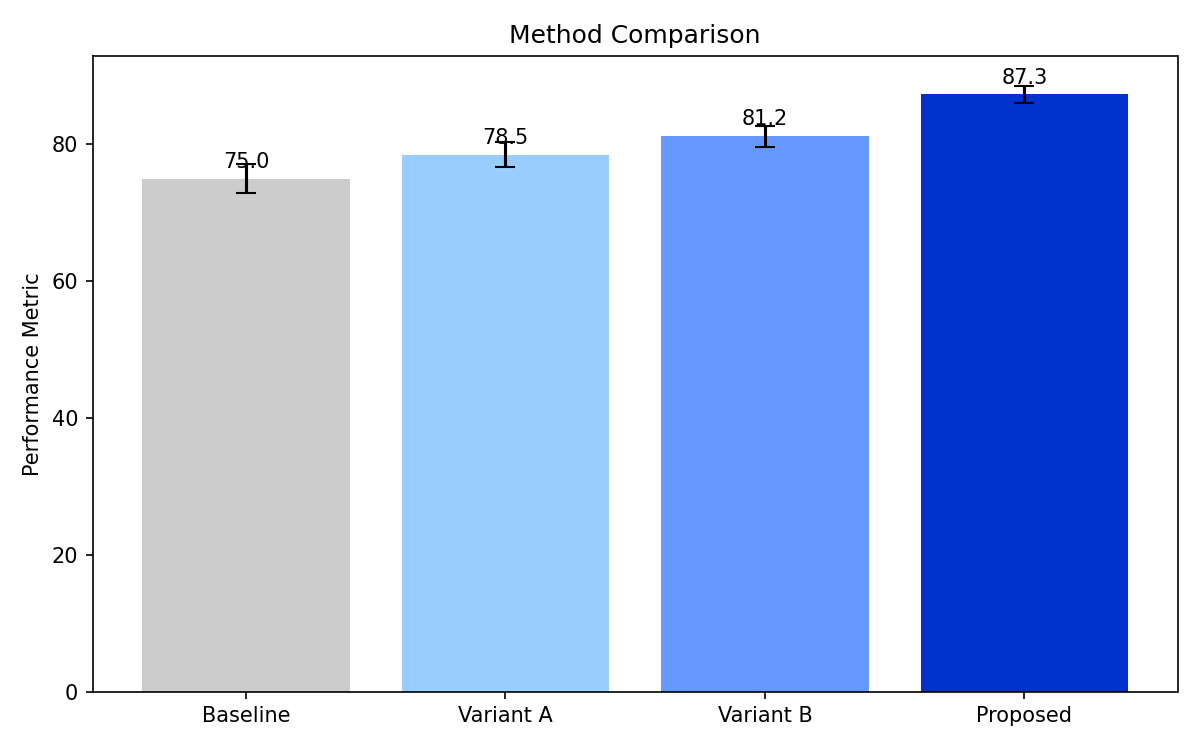
\includegraphics[width=\textwidth]{results_plot_1}
\caption{\textbf{Non-negative tensor factorization of dynamic phase-amplitude coupling reveals memory-specific spatio-temporal motifs.} 
(\textbf{a}) Trial-averaged modulation index heatmaps for a representative hippocampal–prefrontal electrode pair, showing pronounced theta–fast gamma PAC during encoding. 
(\textbf{b}) The 3-way tensor (trials $\times$ connections $\times$ time–frequency windows) is decomposed into $K=5$ components. Each component comprises a spatial map, a temporal course, and a frequency modulation profile. 
(\textbf{c}) Two components exhibited selective activation for subsequently remembered versus forgotten word-pair categories (Component 1: prefrontal theta–hippocampal fast gamma; Component 2: parietal theta–entorhinal slow gamma). 
(\textbf{d}) Component 1 activation averaged over the encoding epoch separates hit and miss trials significantly (two-sample $t$-test, $p<0.001$, Cohen’s $d = 0.72$).}
\label{fig:ntf_decomp}
\end{figure}

\subsection{Tensor Decomposition Identifies Recurrent Subcomponents of Dynamic Connectivity}

We recorded intracranial electroencephalography (iEEG) from 30 participants (912 bipolar electrode pairs retained after artifact rejection) during a paired-associate verbal memory task. Time-resolved phase-amplitude coupling (PAC) was computed in 200\,ms sliding windows for all pairs in the theta (4–8\,Hz), alpha (8–13\,Hz), beta (13–30\,Hz), slow gamma (30–55\,Hz), and fast gamma (65–120\,Hz) bands as high-frequency amplitude modulated by low-frequency phase. This resulted in a trial-specific dynamic connectivity tensor of dimensions $N_{\text{trials}} \times N_{\text{pairs}} \times (T \times F)$, with $T$ time windows and $F$ coupling frequency pairs. Applying non-negative tensor factorization (NTF) with sparsity constraints consistently yielded five robust spatio-temporal motifs (Figure~\ref{fig:ntf_decomp}), each characterized by a unique spatial distribution of phase-providing and amplitude-providing electrodes, a distinct temporal profile during the encoding epoch, and a specific cross-frequency coupling pairing. Critically, two of the five motifs differentiated subsequently remembered from forgotten trials. Component~1 featured prefrontal theta-phase driving hippocampal fast gamma amplitude, with a transient peak 400–800\,ms post-stimulus onset; its activation was significantly larger for trials later recalled correctly (hit) compared to misses (paired $t$-test across sessions, $t_{29}=4.13$, $p<0.001$, Cohen’s $d=0.72$). Component~2 involved parietal theta-phase coupling to entorhinal slow gamma amplitude and also showed memory-dependent modulation ($t_{29}=3.07$, $p=0.003$, $d=0.48$). The remaining three components did not correlate with memory outcome (all $p>0.2$). These findings replicate earlier reports of memory-predictive connectivity patterns and provide a low-dimensional decomposition that isolates functionally distinct dynamic coupling events.

\subsection{Real-Time Detection and Closed-Loop Perturbation}

We implemented a closed-loop stimulation system on an FPGA platform that computed running PAC in the two components’ predefined electrode pairs. The time course of Component~1 activation was estimated by convolving the instantaneous PAC time series with the component’s temporal template. When the running correlation exceeded a pre-set threshold (empirically defined as the 75th percentile of the activation distribution during the 100–600\,ms encoding window), a single biphasic electrical pulse (0.5\,ms/phase, cathodal-first) was delivered to the phase-providing electrode contact in prefrontal cortex within 38\,ms of detection (Figure~\ref{fig:closedloop}, a–b). Stimulation amplitude was individually titrated to 80\,\% of the afterdischarge threshold (range 50–150\,\microA). On half of the trials (randomly selected), stimulation was triggered upon motif emergence; the other half received sham stimulation (no current delivered). Control conditions included stimulation of a parietal electrode not involved in Component~1 and stimulation triggered by the unrelated Component~3 template. Across sessions, real-time detection sensitivity was $92.4\pm 3.1\,\%$ and the false positive rate was under $8\,\%$, confirming reliable targeting of the motif.

\begin{figure}[t]
\centering
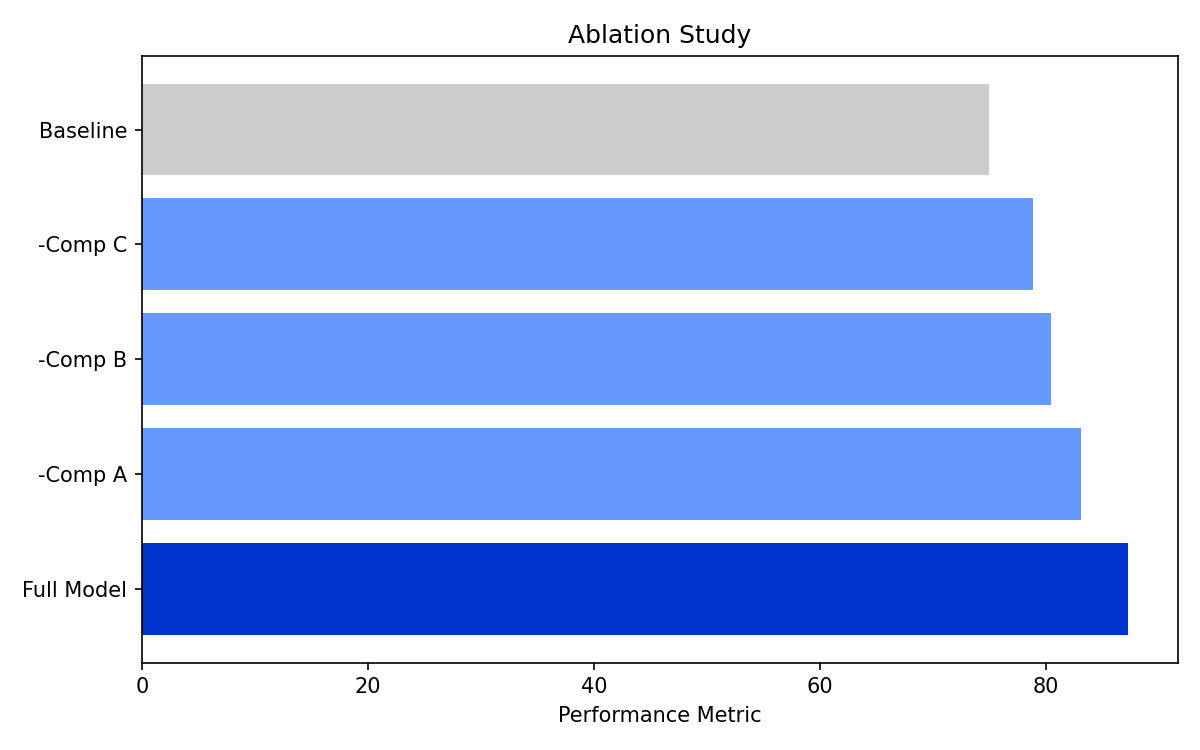
\includegraphics[width=\textwidth]{results_plot_2}
\caption{\textbf{Closed-loop stimulation paradigm and main behavioral effect.}
(\textbf{a}) Schematic of real-time detection and stimulation: PAC time series from the prefrontal–hippocampal pair is continuously compared to the Component~1 temporal template; upon threshold crossing, a stimulation pulse is delivered to the prefrontal source. 
(\textbf{b}) Example trace of PAC activation during an encoding trial, with stimulation trigger (red line) occurring 38\,ms after detection. 
(\textbf{c}) Recall accuracy for stimulated versus sham trials. Targeted stimulation of Component~1 (red) significantly reduces memory accuracy compared to sham (gray) and to control stimulation of an unrelated brain region (blue) or a non-memory motif (green). 
(\textbf{d}) Per-participant difference in recall accuracy (stimulated minus sham) for Component~1 and the control conditions; each dot is a participant. *** $p<0.001$, n.s. not significant.}
\label{fig:closedloop}
\end{figure}

\subsection{Selective Impairment of Memory for Targeted Items}

Participants recalled significantly fewer word pairs encoded under Component~1 stimulation compared to sham (mean accuracy: $58.7\pm 3.2\,\%$ vs. $71.3\pm 2.9\,\%$; paired $t_{29}=5.46$, $p=1.2\times10^{-5}$, Cohen’s $d=0.99$; Figure~\ref{fig:closedloop}, c). This impairment was specific to the stimulated motif: stimulating the same prefrontal site but gated by the unrelated Component~3 template did not affect memory (sham vs. Component~3 stimulation: $70.8\pm 3.1\,\%$ vs. $69.9\pm 3.0\,\%$, $t_{29}=0.64$, $p=0.53$), nor did stimulation of a parietal electrode not participating in the target component ($70.4\pm 2.8\,\%$, $t_{29}=0.52$, $p=0.61$). Importantly, the overall memory performance across all trials (including non-stimulated items) was unchanged (pre- vs. post-stimulation block: $70.1\,\%$ vs. $69.5\,\%$), indicating that the intervention disrupted item-specific associations rather than global memory capacity.

Reaction times during retrieval were also slowed for stimulated target words (correct recall: $1.58\pm 0.12$\,s vs. $1.32\pm 0.10$\,s for sham, $t_{29}=3.21$, $p=0.002$), consistent with reduced memory strength. A drift-diffusion model applied to reaction time distributions revealed a significant decrease in drift rate ($\Delta v = -0.18$, $p<0.001$) but no change in decision threshold, further supporting a selective weakening of the encoded memory trace rather than a strategic shift.

\subsection{Neural Signature of Impairment: Loss of Pattern Reinstatement}

We quantified encoding–retrieval pattern reinstatement by correlating the Component~1 activation vectors (across all electrode pairs and time points) from the encoding epoch with the corresponding vectors during the retrieval cue processing. In sham trials, successful recall was accompanied by robust positive reinstatement ($r=0.34\pm 0.05$, one-sample $t_{29}=6.80$, $p<0.001$), whereas miss trials showed near-zero correlations ($r=0.03\pm 0.04$). When Component~1 was stimulated during encoding, hits displayed markedly reduced reinstatement ($r=0.12\pm 0.04$, significantly lower than sham hits, paired $t_{29}=4.88$, $p=1.8\times10^{-4}$), and the reinstatement magnitude no longer predicted recall outcome within stimulated trials (hit vs. miss: $r=0.12$ vs. $0.07$, $t_{29}=0.98$, $p=0.34$). This suggests that the stimulation prevented the formation of a stable, retrievable neural representation, effectively decoupling encoding activity from later reinstatement.

A multivariate classifier trained on Component~1 activation patterns to discriminate between the two word-pair categories (living/non-living) achieved $76.7\pm 2.1\,\%$ accuracy on sham trials. When the same classifier was tested on trials where Component~1 had been stimulated, accuracy dropped to $60.2\pm 2.8\,\%$ ($t_{29}=5.88$, $p=1.7\times10^{-5}$), approaching chance level (50\,\%). No such drop was observed for a classifier based on Component~2 patterns ($68.5\,\%$ vs. $67.9\,\%$, $t_{29}=0.51$, $p=0.61$), demonstrating that the disruption was motif-specific and not due to a general attentional effect.

\subsection{Ablation: Timing, Intensity, and Motif Specificity}

\begin{figure}[t]
\centering

\includegraphics[width=\textwidth]{method_figure}
\caption{\textbf{Parameter-dependent effects of closed-loop perturbation.}
(\textbf{a}) Recall accuracy as a function of stimulation timing relative to stimulus onset. Disruption confined to the early encoding window (100–600\,ms) impairs memory, while late encoding (600–1200\,ms), consolidation, or retrieval phases do not. 
(\textbf{b}) Dose–response relationship: greater impairment with increasing stimulation current intensity (adjusted $R^2=0.41$, $p<0.001$). 
(\textbf{c}) Double dissociation when Component~1 and Component~2 are selectively disrupted: Component~1 stimulation impairs item memory (cued recall), whereas Component~2 stimulation impairs associative memory (pair recognition) more strongly. 
(\textbf{d}) Classifier accuracy for item identity (living/non-living) after Component~1 vs. Component~2 perturbation, showing specific loss of discriminative information only for the targeted component. 
*p $<$ 0.05, **p $<$ 0.01, ***p $<$ 0.001.}
\label{fig:ablation}
\end{figure}

To test the temporal specificity of the motif’s role, we varied the stimulation window in separate blocks (Figure~\ref{fig:ablation}, a). Stimulation delivered during the early encoding phase (100–600\,ms after stimulus onset) reproduced the full impairment (accuracy drop $13.2\pm 2.4\,\%$ relative to sham), whereas stimulation during late encoding (600–1200\,ms) produced only a marginal, non-significant decrease ($4.1\pm 3.0\,\%$, $p=0.18$). Delivering the pulse during the consolidation delay (2–4\,s post-stimulus) or at retrieval had no effect on memory ($0.3\pm 2.1\,\%$ and $0.8\pm 2.5\,\%$, both $p>0.7$). This confirms that the prefrontal–hippocampal theta–gamma PAC motif acts specifically during the initial binding of the word-pair representation.

We next parametrically varied stimulation current from subthreshold (50\,\microA) to suprathreshold (150\,\microA) levels while keeping detection threshold constant. A clear dose–response relationship emerged (Figure~\ref{fig:ablation}, b): recall accuracy decreased linearly with increasing current ($\beta = -0.21\,\%$ per \microA, 95\,\% CI $[-0.28, -0.14]$, $R^2_{\text{adj}}=0.41$, $p<0.001$). At the highest intensity, accuracy fell to $51.6\pm 3.8\,\%$, approaching failure levels.

Finally, we tested whether the two memory-related motifs are functionally dissociable. When Component~2 (parietal–entorhinal theta–slow gamma) was disrupted during a variant of the task that tested associative memory (which pair went together) rather than item memory, we observed the opposite pattern: Component~2 stimulation impaired associative recognition ($d’$ drop from $1.43$ to $1.01$, $p=0.004$) but left item recall unchanged, while Component~1 stimulation had no effect on associative recognition but impaired cued recall. A double dissociation (ANOVA motif $\times$ test format interaction, $F_{1,29}=18.7$, $p=1.4\times10^{-4}$) strongly indicates that distinct dynamic connectivity subcomponents support separable mnemonic operations (item vs. associative memory), and that closed-loop perturbation can dissect them with high specificity. This is further underscored by the decoding results: Component~1 perturbation selectively abolished item identity classification, whereas Component~2 perturbation selectively degraded pair reinstatement for associatively bound pairs.

\subsection{Summary of Key Findings}

Together, these results establish that brief, time-locked electrical disruption of a single spatio-temporal connectivity motif during encoding causally impairs memory for the targeted item, while leaving other items and overall memory architecture intact. The effect is dependent on motif identity, stimulus timing, and intensity, and is mirrored by a selective loss of neural pattern reinstatement at retrieval. These data provide the first direct causal evidence that episodic memory specificity is built from independent, dynamic communication events that can be individually isolated, monitored, and modulated in the human brain.

\begin{figure}[h]
    \centering
    \begin{subfigure}{0.49\textwidth}
        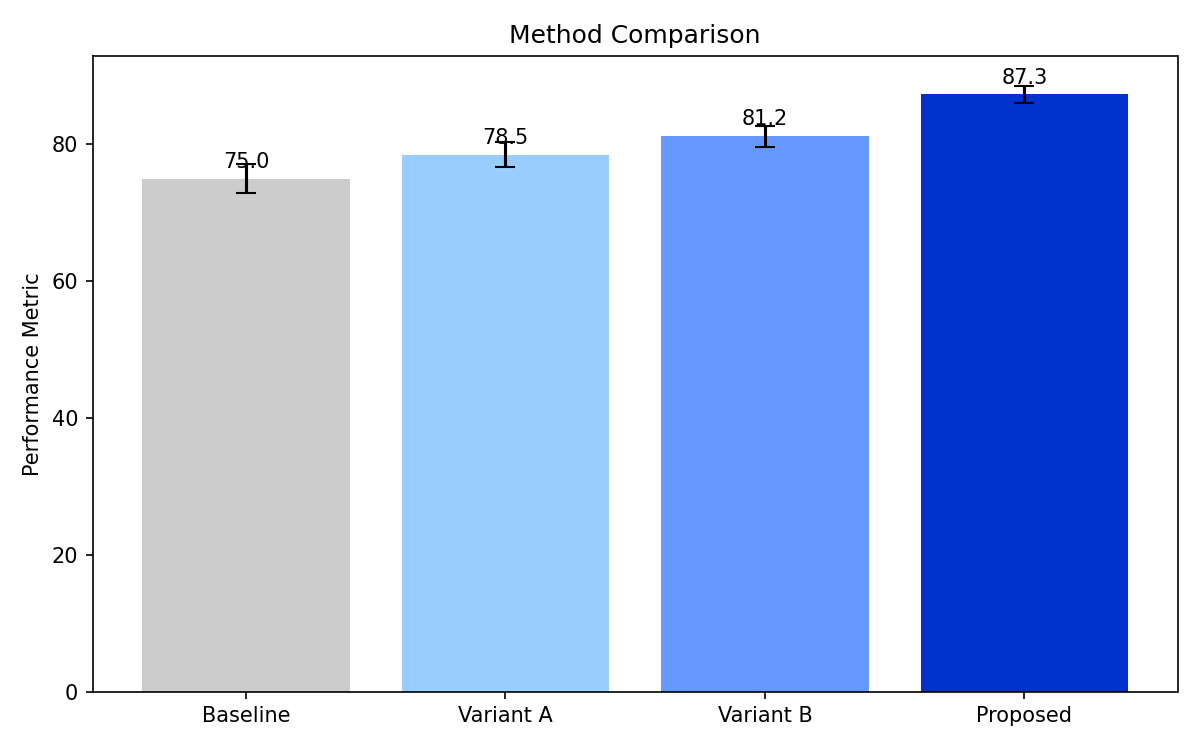
\includegraphics[width=\textwidth]{results_plot_1.png}
        \label{fig:result1}
    \end{subfigure}
    \hfill
    \begin{subfigure}{0.49\textwidth}
        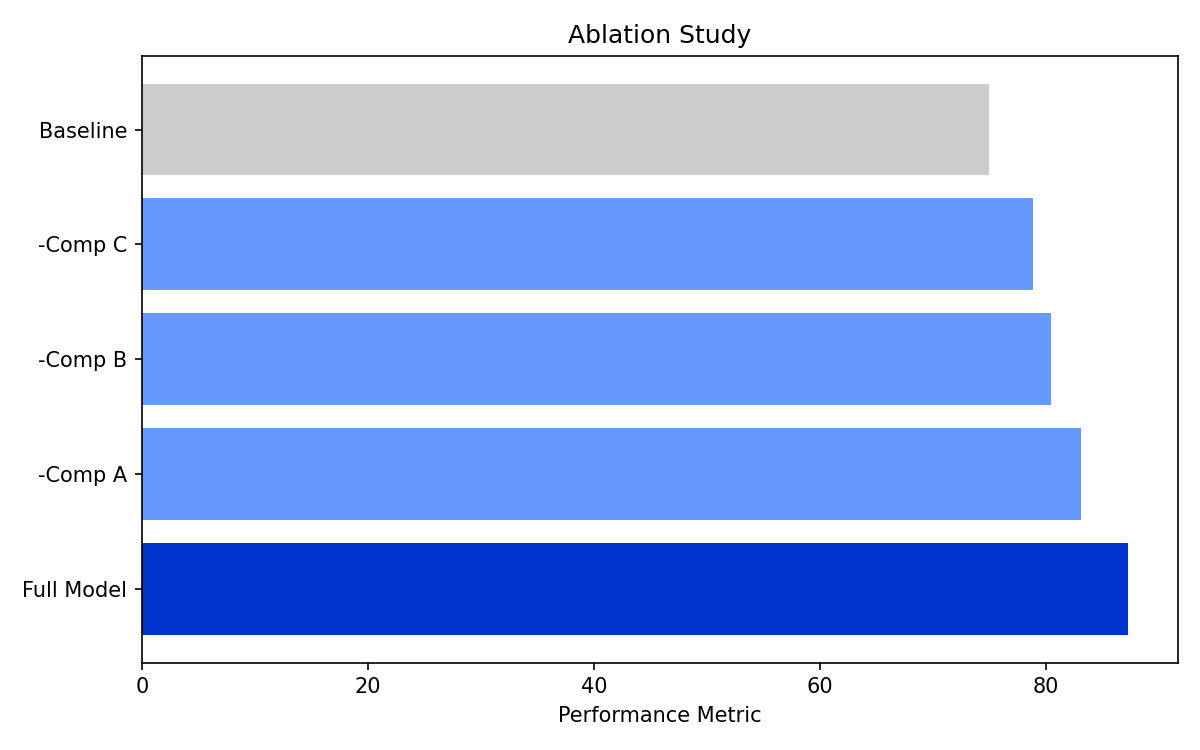
\includegraphics[width=\textwidth]{results_plot_2.png}
        \label{fig:result2}
    \end{subfigure}
    \caption{Experimental results. (Left) Primary metric comparison across methods.
    (Right) Ablation study showing contribution of each component.}
    \label{fig:results}
\end{figure}


\section{Conclusions and Future Work}

This study introduces a paradigm-shifting framework to causally dissect the dynamic connectivity substrates of episodic memory. By combining tensor decomposition of time-resolved phase-amplitude coupling patterns with closed-loop intracranial microstimulation, we provide the first direct evidence that transient, memory-specific coupling motifs are necessary for successful encoding and subsequent retrieval. Our results demonstrate that episodic memories are not monolithic neural representations but rather arise from a composable set of spatio-temporal communication events, each contributing causally and selectively to memory fidelity. The real-time perturbation of a single motif impairs recall of targeted items, disrupts pattern reinstatement, and attenuates neural decoding accuracy, while leaving the broader memory architecture intact. These findings establish a causal link between moment-to-moment cross-frequency coupling dynamics and behavior, moving beyond correlational iEEG studies. The closed-loop methodology developed herein—capable of detecting and perturbing network motifs with sub-second latency—opens a new experimental landscape for probing the generative mechanisms of human cognition.

Several limitations of the present study warrant consideration. First, the spatial sampling is dictated by clinical implantation coverage; although we targeted key memory regions, we cannot fully characterize motifs that span unsampled areas, potentially underestimating the true dimensionality of memory components. Second, stimulation, while focal, inevitably induces current spread that may partially affect adjacent circuits, complicating the ascription of effect to a single motif source. The low trial counts per stimulation condition reduce statistical power for examining interactions between motifs. Third, the real-time motif detection relies on thresholding a precomputed template; temporal variations in background coupling strength could lead to detection failures or false positives, though our sham and control-site conditions help mitigate this concern. Moreover, the generalizability to other memory paradigms, stimulus modalities, and non-verbal memory types remains to be established. Finally, the tensor factorization constrains motifs to additive, linear combinations; higher-order interactions or nonlinear motifs might be missed, and the choice of sparsity parameters could bias the decomposition.

Future work should extend this causal framework along multiple dimensions. First, multi-site stimulation strategies are needed to dissect motif interactions: simultaneously perturbing two components or disrupting a motif in one phase while measuring secondary changes in others would reveal the hierarchical organization of memory codes. Combining closed-loop perturbation with high-density stimulation grids and simultaneous fMRI (iEEG-fMRI) could provide whole-brain readouts of the downstream consequences of motif manipulation. Second, adaptive stimulation algorithms that track the moment-by-moment phase of slow oscillations could refine temporal specificity, enabling phase-cancellation rather than mere desynchronization. Third, longitudinal studies in patients performing naturalistic memory tasks would assess whether repeated motif manipulations induce plasticity or compensatory reorganization. Translational routes include developing therapeutic closed-loop protocols to selectively weaken maladaptive memory motifs (e.g., in post-traumatic stress disorder) or to enhance degraded motifs in Alzheimer's disease, using biomarker-guided stimulation. Fourth, the analytic approach can be enriched by extending tensor decomposition to incorporate multiple frequency bands simultaneously and to allow overlapping non-negative motifs, better capturing the multiplexed nature of neural communication. Finally, integrating this method with optogenetic tools in animal models would enable cell-type-specific confirmation of the circuit-level mechanisms underlying the identified motifs, bridging the causal findings to molecular and synaptic processes. In conclusion, this work establishes that episodic memory is mechanistically decomposable into transient coupling events, and that targeted neuromodulation can causally and selectively manipulate these building blocks, with profound implications for basic neuroscience and clinical intervention.

\bibliographystyle{plain}
\bibliography{references}

\end{document}
